\documentclass{article}
\usepackage{graphicx} % Required for inserting images
\usepackage{amsmath}
\usepackage{hyperref}
\usepackage{amsthm}
\usepackage{amssymb}
\title{Benchmarking: Schrodinger Bridge Estimator vs Trajectory Inference
}
\author{Viresh Pati}
\date{February 2025}

\begin{document}

\maketitle

\section{Plug-in Estimation of Schrodinger Bridges}
\subsection{Single-snapshot}
Single snapshot $\mu \rightarrow \nu$ is the natural use case. One entropic OT (Sinkhorn) solve yields dual potentials which define a drift form $\mu $ to $\nu$.
\subsection{Benchmark} 
Often BW-UVP or a second-moment metric checks how well the final distribution matches $\nu$ (especially for high-dimensional tasks like $\mathbb{R}^{64}$ .
\subsection{Multi-time data}
Not directly addressed. We could only bridge the first and last timepoints, ignoring intermediate snapshots.
\section{Trajectory Inference via Mean-field Langevin}
\subsection{Multiple Snapshots}
Iteratively solves Schrodinger Bridges between consecutive timpoints $(u_{t_1},...u_{t_{T}})$
\subsection{Benchmark}
Typically Energy Distance or 2-Wasserstein distance at each snapshot. Can handle branching/growth.
\subsection{Two-snapshot scenario}
MFL can still run but it may be more complex than needed for a single step from $\mu$ to $\nu$ 
\section{Cross-Comparison Strategy}
\subsection{Setup}
\subsubsection{D1 (Two-snapshot)}
You only have a source and target distribution. This is the setting in JNW paper.
\subsubsection{D2 (Multi-time)}
You have multiple snapshots $u_{t_1},...,u_{t_T}$. This is the setting in   Mean-field Langevin paper.
\subsubsection{Parameters}
Some hyperparameters are taken differently from reference paper.

\subsection{Methods}
\subsubsection{Plug-in (Entropic OT)}
\begin{itemize}
    \item A single Sinkhorn run between $\mu$ and $\nu$
    \item Minimal iteration cost: once the EOT potentials are found you plug into a drift
    \item Measure final accuracy with BW-UVP
\end{itemize}
\subsubsection{Mean-Field Langevin}
\begin{itemize}
    \item Iteratively solves Schrodinger Bridges between consecutive snapshots.
    \item Higher computational cost by repeating multiple OT subproblems
    \item Measures multi-time accuracy e.g. Energy Distance to each snapshot

\end{itemize}
\subsection{Discussion}
A few notes regarding the off-diagonal cases. 
\begin{itemize}
\item Using MFL is perfectly fine for a two-snapshot problem (and I imagine could perform better in some scenarios) but comes with additional computation. 
\item However, in a multi-time scenario, using the plug-in estimator probably struggles. Technically, each iteration of MFL takes the current guess of each marginal, runs multiple sinkhorn iterations, and updates each $\mu^{ti}$ by a gradient-descent like step in the distribution space which depends on those bridging potentials. 
\item  A naive approach to applying the plug-in estimator might be (1) solve an EOT subproblem from $\mu_t$ to $\mu_{t+1}$ (2) plug in the resulting drift (3) Repeat
\item \textbf{Issue:} once you change the marginal $\mu_{ti}$ by adjusting it via a plug-in drigt from earlier times, that might alter the correct bridging for the next time slice. You'd have to do multiple rounds of re-checking the global solution. This is probably a research direction.
    
\end{itemize}

\section{Results }
\subsection{Plug-in Estimator}
\subsubsection{Two Marginals Case}
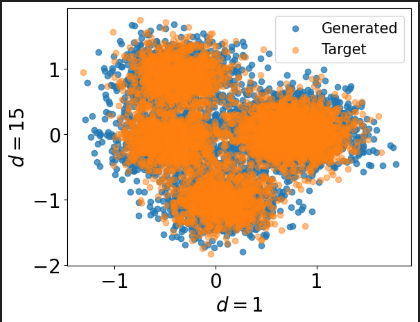
\includegraphics[width=\textwidth, height=0.4\textheight]{Smooth Schrodinger Bridges/benchmark-results/PluginEstimatorNative.png}
\textbf{Speed:} $45.6 s \pm302ms$ per loop (mean $\pm $ std. dev. of 7 runs, 1 loop each)\\
\textbf{Accuracy:} BW-UVP = 0.372 (paper is $0.41\pm0.03$)
\subsubsection{Multi-time Case }
\textbf{Speed:}\\
\textbf{Accuracy:}
\subsection{Mean-field Langevin}
\subsubsection{Two Marginals Case}
This is not of any relevance. There is hardly any reason to attempt MFL on 2-marginal cases, since we have a much more efficient plug-in estimator. Some basic tests I ran confirmed this.\\
Total simulation time for 2500 iterations: 2.8342 seconds\\
Average time per iteration: 0.001134 seconds\\
Final BW-UVP distance: 0.4102


\subsubsection{Multi-Time Case }
\textbf{Speed:} Between 80-120 seconds per run depending on choice of hyperparameters for mfl runs, 4-6 seconds gwot runs. Note that gwot requires around 100x less iterations. in Figure 1\\
\textbf{Accuracy:}\\
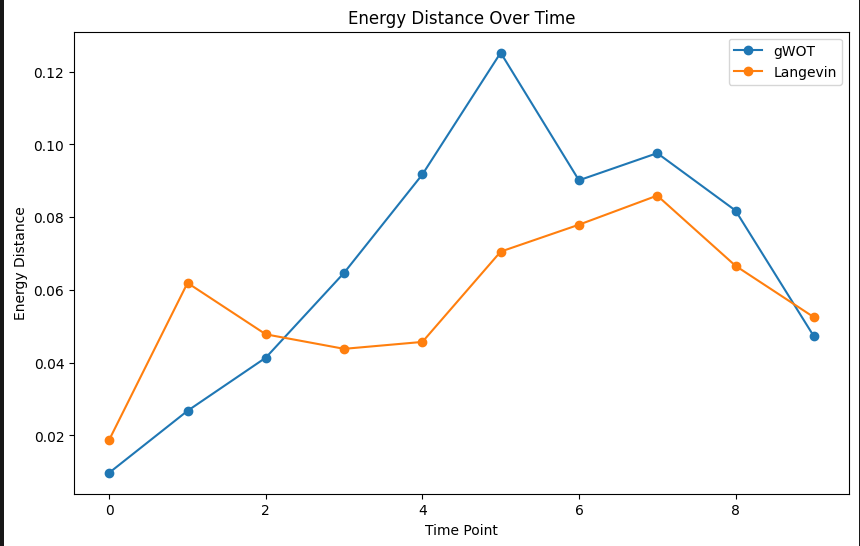
\includegraphics[width=\textwidth, height=0.4\textheight]{Smooth Schrodinger Bridges/benchmark-results/LangevinNativePlot.png}\\
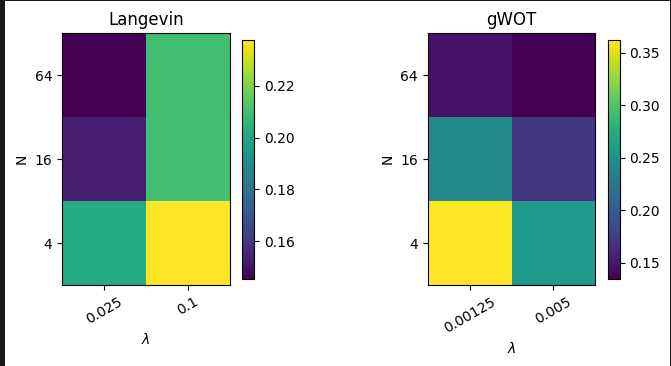
\includegraphics[width=\textwidth, height=0.4\textheight]{Smooth Schrodinger Bridges/benchmark-results/LangevinNativePlot2.png}\\
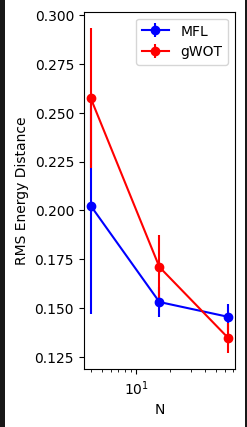
\includegraphics[width=\textwidth, height=\textheight]{Smooth Schrodinger Bridges/benchmark-results/LangevinNativePlot3.png}
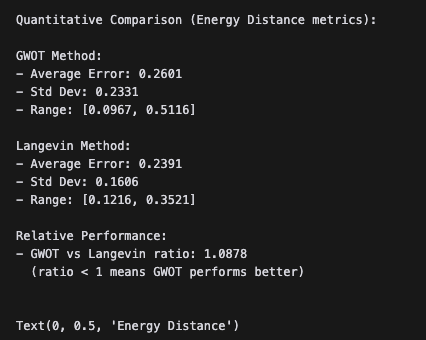
\includegraphics[width=\textwidth, height=0.4\textheight]{Smooth Schrodinger Bridges/benchmark-results/LangevinNativeQuant.png}

\end{document}
